
\subsection{Example of dynamic HPFC on simple snake robot}

This section shows a very simple scenario with a 2-link robot and one obstacle. The aim is to provide a better understanding of the theory presented in \ref{subsec:DHPFC} and show the structure of the various mapping matrices.
Furthermore, the example shows the necessity of using simulation software to study more intricate cases, as the matrices for this simple case already get quite complex.

The configuration of the robot and its environment is illustrated in Figure \ref{fig:ex_2link}. %To make the example as simple as possible, the robot is still in the given configuration and all velocities are thus zero.
The mass of each link is $m = 1 kg$ and the link length is $l=1 m$. The value of the joint angles $\phi_0$ and $\phi_1$ are $0$ and $\pi/2$ respectively.

\begin{figure}
    \centering
    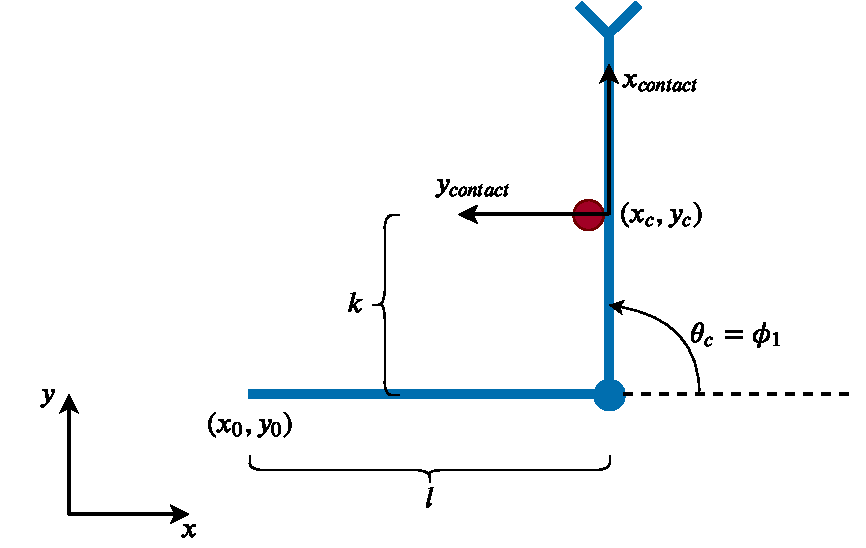
\includegraphics[width=0.9\textwidth]{figures/theory/example_2link.pdf}
    \caption{Model of 2-link snake robot}
    \label{fig:ex_2link}
\end{figure}

The joint variables are given by

\begin{equation}
    \mathbf{q} =
    \begin{bmatrix}
        \phi_0 & \phi_1 & x_0 & y_0 & k & \phi_c
    \end{bmatrix}^T \in \mathcal{R}^5.
\end{equation}
\\
The task coordinates by the contact point are given by

\begin{equation}
    \mathbf{r}_t = 
    \begin{bmatrix}
        x_c & y_c & \theta_t
    \end{bmatrix}^T \in \mathcal{R}^3,
\end{equation}
\\
where $\theta_t$ in the given configuration is the sum of the two joint angles $\phi_0$ and $\phi_1$. Furthermore, the constraint coordinates, which should always remain constant, are given by

\begin{equation}
    \mathbf{r}_c = 
    \begin{bmatrix}
        x_c & y_c & \theta_c
    \end{bmatrix}^T \in \mathcal{R}^3,
\end{equation}
\\
where $\theta_c$ is the angle of the obstacle point coordinate system in the base frame. This angle should always be zero, as can be seen from Figure \ref{fig:ex_2link}. It should be noted that the origin of the two frames, described by $(x_c, y_c)$, is the same. This is a result of the contact point and obstacle being modeled as a single point.

Lastly, the velocities and forces represented in the task frame (visualized in Figure \ref{fig:ex_2link} as $(x_t, y_t)$) are 

\begin{equation}
    \mathbf{v} =
    \begin{bmatrix}
        v_x & v_y
    \end{bmatrix}^T \in \mathcal{R}^2,
\end{equation}

\begin{equation}
    \mathbf{f} =
    \begin{bmatrix}
        f_x & f_y
    \end{bmatrix}^T \in \mathcal{R}^2.
\end{equation}
\\

\subsubsection{Dynamics}

The dynamics of this robot can be found using the Euler-Lagrange method described in \ref{sec:dyn}.
The position and velocities of the middle of the links in the base frame are

\begin{equation}
    \begin{split}
        p_0 &=
        \begin{bmatrix}
            x_0 + l/2 cos(\phi_0)\\
            y_0 + l/2 sin(\phi_0)
        \end{bmatrix}, \\
        p_1 &=
        \begin{bmatrix}
            x_0 + l cos(\phi_0) + l/2 cos(\phi_0+ \phi_1)\\
            y_0 + l sin(\phi_0) + l/2 sin(\phi_0+\phi_1)
        \end{bmatrix},
    \end{split}
\end{equation}

\begin{equation}
    \begin{split}
        \dot{p}_0 &=
        \begin{bmatrix}
            \dot{x_0} - l/2 \dot{\phi_0} sin(\phi_0)\\
            \dot{y_0} + l/2 \dot{\phi_0} cos(\phi_0)
        \end{bmatrix}, \\
        \dot{p}_1 &=
        \begin{bmatrix}
            \dot{x_0} - l \dot{\phi_0} sin(\phi_0) - l/2 (\dot{\phi}_0 +\dot{\phi}_1) sin(\phi_0+\phi_1)\\
            \dot{y_0} + l \dot{\phi_0} cos(\phi_0) + l/2 (\dot{\phi}_0 +\dot{\phi}_1) cos(\phi_0+\phi_1)
        \end{bmatrix}.
    \end{split}
\end{equation}
\\
The Lagrangian and the dynamical equations can now be calculated from (\ref{eq:ex_dyn1}) and (\ref{eq:ex_dyn2}), where $I = (1/12)ml^2 = 1/12$.

\begin{equation}\label{eq:ex_dyn1}
    \begin{split}
        L &= K_{translational,0} + K_{rotational,0} + K_{translational,1} + K_{rotational,1}\\
        &= \frac{1}{2} m \dot{p}_0^2 + \frac{1}{2}I\dot{\phi_0}^2 + \frac{1}{2} m \dot{p}_1^2 + \frac{1}{2}I\dot{\phi_1}^2
    \end{split}
\end{equation}
\\
\begin{equation}\label{eq:ex_dyn2}
    \boldsymbol{\tau} = \frac{d}{dt} \frac{\partial L}{\partial \dot{\mathbf{q}}} - \frac{\partial L}{\partial \mathbf{q}}
\end{equation}
\\
Inserting the values for the constants $m$ and $l$ and comparing the result to the form given in (\ref{eq:eom}) gives the inertia and Coriolis matrix in (\ref{eq:ex_inertia}) and (\ref{eq:ex_coriolis}) respectively. The trigonometric functions are abbreviated to $s_0 = sin(\phi_0)$, $s_1 = sin(\phi_1)$, $c_0 = cos(\phi_0)$, $c_1 = cos(\phi_1)$, $s_{01} = sin(\phi_0+\phi_1)$ and $c_{01} = cos(\phi_0+\phi_1)$.

\begin{equation}\label{eq:ex_inertia}
    \mathbf{M(q)} = 
    \begin{bmatrix}
        c_1+\frac{5}{3} & \frac{c_1}{2} + \frac{1}{3} & -\frac{s_{01}}{2} - \frac{3s_0}{2} & \frac{c_{01}}{2} + \frac{3c_0}{2} & 0 & 0 \\
        \frac{c_1}{2}+\frac{1}{3} & \frac{1}{3} & -\frac{s_{01}}{2} & \frac{c_{01}}{2} & 0 & 0 \\
        -\frac{s_{01}}{2}- \frac{3s_0}{2} & -\frac{s_{01}}{2} & 2 & 0 & 0 & 0 \\
        \frac{c_{01}}{2}+ \frac{3c_0}{2} & \frac{c_{01}}{2} & 0 & 2 & 0 & 0 \\
        0 & 0 & 0 & 0 & 0  & 0 \\
        0 & 0 & 0 & 0 & 0  & 0
    \end{bmatrix}
\end{equation}

\begin{equation}\label{eq:ex_coriolis}
    \mathbf{C(q, \dot{q})} = 
    \begin{bmatrix}
        -\frac{\dot{\phi}_1 s_1 (2\dot{\phi}_0+ \dot{\phi}_1)}{2} \\
        \frac{\dot{\phi}_0^2 s_1}{2} \\
        -\frac{3 \dot{\phi}_0^2 c_1}{2} - \frac{\dot{\phi}_0^2 c_{01}}{2} - \frac{\dot{\phi}_1^2 c_{01}}{2} - \dot{\phi}_0 \dot{\phi}_1 c_{01} \\
        -\frac{3 \dot{\phi}_0^2 s_1}{2} - \frac{\dot{\phi}_0^2 s_{01}}{2} - \frac{\dot{\phi}_1^2 s_{01}}{2} - \dot{\phi}_0 \dot{\phi}_1 s_{01} \\
        0 \\ 0
    \end{bmatrix}
\end{equation}
\\
Inserting the given angles significantly simplifies the matrices to

\begin{equation}
    \mathbf{M} = 
    \begin{bmatrix}
        5/3 & 1/3 & -1/2 & 3/2 & 0& 0 \\
        1/3 & 1/3 & -1/2 & 0 & 0 & 0\\
        -1/2 & -1/2 & 2 & 0 & 0 & 0\\
        3/2 & 0 & 0 & 2 & 0 & 0\\
        0 & 0 & 0 & 0 & 0 & 0\\
        0 & 0 & 0 & 0 & 0 & 0
    \end{bmatrix}
\end{equation}

\begin{equation}
    \mathbf{C(\dot{q})} = 
    \begin{bmatrix}
        -(\dot{\phi}_1 (2\dot{\phi}_0+ \dot{\phi}_1))/2 \\
        \dot{\phi}_0^2/2 \\
        0 \\
        -3 \dot{\phi}_0^2/2 - \dot{\phi}_0^2/2 - \dot{\phi}_1^2/2 - \dot{\phi}_0 \dot{\phi}_1 \\
        0 \\ 0
    \end{bmatrix}.
\end{equation}

\subsubsection{Constraints}

The single obstacle present in this example stands for the single constraint on the snake robot. 
From \ref{subsec:DHPFC} it is known that the constraint is on the velocity of the contact point normal to the link in contact. This velocity is here given as

\begin{equation}
    v_y = - sin(\theta_t) \dot{x}_c + cos(\theta_t) \dot{y}_c
\end{equation}
\\
In order for the link to both stick to the obstacle and not penetrate it, the velocity $v_y$ should be zero. This constraint is put on the form in (\ref{eq:hpfc:derhypsurf}) and the given angles are inserted.

\begin{equation}\label{eq:ex_EF}
    \mathbf{E}_F = 
    \begin{bmatrix}
        - sin(\theta_t) & cos(\theta_t) & 0
    \end{bmatrix}
    =
    \begin{bmatrix}
        - 1 & 0 & 0
    \end{bmatrix}
\end{equation}
\\
The derivative of (\ref{eq:ex_EF}) is
\begin{equation}\label{eq:ex_EFd}
    \mathbf{\dot{E}}_F = 
    \begin{bmatrix}
        -cos(\theta_t) \dot{\theta}_t & - sin(\theta_t) \dot{\theta}_t & 0
    \end{bmatrix}
    \begin{bmatrix}
        0 & -\dot{\theta}_t & 0
    \end{bmatrix}.
\end{equation}
\\
Inserting (\ref{eq:ex_EFd}) into (\ref{eq:dhpfc_arf}) gives
\begin{equation}
    a_{rF} = -\dot{\theta}_t \dot{y}_c.
\end{equation}
\\
It is however known that the obstacle itself cannot move. This, together with the obstacle being modeled as a point, results in the velocity of the contact point being zero at all times. Thus $a_{rF}=0$.

(\ref{eq:dhpfc_EPi}) and (\ref{eq:dhpfc_E}) give
\begin{equation}
    \mathbf{E}_P = 
    \begin{bmatrix}
        cos(\theta_t) & sin(\theta_t) & 0 \\
        0 & 0 & 1
    \end{bmatrix}=
    \begin{bmatrix}
        0 & 1 & 0 \\
        0 & 0 & 1
    \end{bmatrix},
\end{equation}
\begin{equation}
    \mathbf{E}=
    \begin{bmatrix}
        0 & 1 & 0 \\
        0 & 0 & 1 \\
        -1 & 0 & 0
    \end{bmatrix}.
\end{equation}
\\
The task coordinates can be expressed as
\begin{equation}
    \mathbf{r}_t =
    \begin{bmatrix}
        x_0 + l cos(\phi_0) + k cos(\phi_0+\phi_1)\\
        y_0 + l sin(\phi_0) + k sin(\phi_0+\phi_1)\\
        \phi_0+\phi_1
    \end{bmatrix}.
\end{equation}
\\
The corresponding Jacobian an its derivative can thus be calculated to
\begin{equation}
    \begin{split}
        \mathbf{J}_t&=
        \begin{bmatrix}
            -l s_0 - k s_{01} & - k s_{01} & 1 & 0 & c_{01} & 0 \\
            l c_0 + k c_{01} & k c_{01} & 0 & 1 & s_{01} & 0 \\
            1 & 1 & 0 & 0 & 0 & 0
        \end{bmatrix}\\&=
        \begin{bmatrix}
            - k & - k & 1 & 0 & 0 & 0 \\
            1 &0 & 0 & 1 & 1 & 0 \\
            1 & 1 & 0 & 0 & 0 & 0
        \end{bmatrix},
    \end{split}
\end{equation}
\begin{equation}\label{eq:ex_Jd}
    \begin{split}
        \mathbf{\dot{J}}_t&=
        \begin{bmatrix}
            - \dot{k} s_{01} -l \dot{\phi}_0c_0 -k c_{01}(\dot{\phi_0}+\dot{\phi_1}) & -\dot{k} s_{01}-k c_{01}(\dot{\phi_0}+\dot{\phi_1}) & 0 & 0 & -s_{01}(\dot{\phi_0}+\dot{\phi_1})  & 0\\
            \dot{k} c_{01} -l \dot{\phi}_0s_0 -k s_{01}(\dot{\phi_0}+\dot{\phi_1}) & \dot{k} c_{01}-k s_{01}(\dot{\phi_0}+\dot{\phi_1}) & 0 & 0 & c_{01}(\dot{\phi_0}+\dot{\phi_1}) & 0 \\
            0 & 0 & 0 & 0 & 0 & 0
        \end{bmatrix}\\&=
        \begin{bmatrix}
            - \dot{k} -\dot{\phi}_0 & -\dot{k} & 0 & 0 & -(\dot{\phi_0}+\dot{\phi_1}) & 0 \\
            -\dot{k}(\dot{\phi_0}+\dot{\phi_1}) & -\dot{k}(\dot{\phi_0}+\dot{\phi_1}) & 0 & 0 & 0 & 0\\
            0 & 0 & 0 & 0 & 0 & 0
        \end{bmatrix}.
    \end{split}
\end{equation}
\\
Inserting (\ref{eq:ex_Jd}) into (\ref{eq:dhpfc_aq}) gives
\begin{equation}
    \mathbf{a}_q =
    \begin{bmatrix}
            - (\dot{k} +\dot{\phi}_0)\dot{\phi}_0 -\dot{k} \dot{\phi}_1 -(\dot{\phi_0}+\dot{\phi_1})\dot{k} \\
            -\dot{k}(\dot{\phi_0}+\dot{\phi_1})\dot{\phi}_0 -\dot{k}(\dot{\phi_0}+\dot{\phi_1})\dot{\phi}_1 \\
            0
        \end{bmatrix}.
\end{equation}

\subsubsection{Calculation of the control torque}

All matrices necessary to derive the control torque are now defined. To make the calculation of the torque even simpler, the static case where all velocities are zero is considered. The result is calculated using (\ref{eq:dhpfc_tau_c})-(\ref{eq:dhpfc_qddd}) and a desired force $f_F = 1 N$ and desired acceleration $\ddot{\mathbf{r}}_d = [0, 0, 1 rad/s^2]^T$. \hl{Quite fast rotation and light force?}

\begin{equation}
    \mathbf{\ddot{q}}_d =
    \begin{bmatrix}
        0 & \frac{1}{5} & \frac{2}{5}\\
        0 & -\frac{1}{5} & \frac{3}{5}\\
        1 & 0 & k \\
        0 & \frac{2}{5} & -\frac{1}{5}\\
        0 & \frac{2}{5} & -\frac{1}{5} \\
        0 & 0 & 0
    \end{bmatrix}\left\{
    \begin{bmatrix}
        0 & 0 & -1\\
        1 & 0 & 0\\
        0 & 1 & 0
    \end{bmatrix}
    \begin{bmatrix}
        0\\   1\\   0
    \end{bmatrix}-
    \begin{bmatrix}
        0\\   0\\   0
    \end{bmatrix}\right\}=
    \begin{bmatrix}
        \frac{2}{5}\\
        \frac{3}{5}\\
        k \\
        -\frac{1}{5}\\
        -\frac{1}{5} \\
        0
    \end{bmatrix}
\end{equation}
\\
The distance $k$ from the joint to the obstacle is chosen to be $1/2 m$.
\begin{equation}
    \boldsymbol{\tau}_P = 
    \begin{bmatrix}
        5/3 & 1/3 & -1/2 & 3/2 & 0 & 0 \\
        1/3 & 1/3 & -1/2 & 0 & 0 & 0 \\
        -1/2 & -1/2 & 2 & 0 & 0 & 0 \\
        3/2 & 0 & 0 & 2 & 0 & 0 \\
        0 & 0 & 0 & 0 & 0  & 0\\
        0 & 0 & 0 & 0 & 0  & 0
    \end{bmatrix}
    \begin{bmatrix}
        2/5\\
        3/5\\
        k \\
        -1/5\\
        -1/5\\0
    \end{bmatrix}=
    \begin{bmatrix}
        0.3167\\
        0.0833\\
        0.5000 \\
        0.2000\\
        0\\0
    \end{bmatrix}
\end{equation}

\begin{equation}
    \boldsymbol{\tau}_F = 
    \begin{bmatrix}
       -k & 1 & 1\\
       -k & 0 & 1\\
       1 & 0 & 0\\
       0 & 1 & 0\\
       0 & 1 & 0 \\
       0 & 0 & 0
    \end{bmatrix}
    \begin{bmatrix}
        -1 \\ 0 \\ 0
    \end{bmatrix}=
    \begin{bmatrix}
       0.5000\\
       0.5000\\
       -1.000\\
       0.000\\
       0.000\\ 0
    \end{bmatrix}
\end{equation}

\begin{equation}
    \boldsymbol{\tau}_c =
    \begin{bmatrix}
        0.8167 & 0.5833 & -0.5000 & 0.2000 & 0.000 & 0.000
    \end{bmatrix}^T
\end{equation}

\hl{Discuss this result. The torques to the translational positions cannot be applied. Is this what the servo feedback thing is for?? only tau 1 can really be applied. k ends up being a free variable!}